\documentclass[../../doc.tex]{subfiles}
\graphicspath{{\subfix{../../img}}}
\begin{document}
    \subsection{Планарная модель руки, держащей предмет}
    
    Рассмотрим руку человека, держащего стержень.
    В некотором приближении можно считать, что мы имеем трехсекционный математический маятник.
    Для каждого из $3$-x сочленений нам известны:
    \begin{enumerate}\itemsep0em 
        \item Масса сочленения $m_i$, $i=1,2,3$;
        \item Линейная плотность сочленения $\rho_i = \rho_i(x)$, $0 \leqslant x \leqslant l_i$, $i=1,2,3$;
        \item Длина сочленения $l_i$, $i=1,2,3$;
        \item Угол поворота сочленения $\theta_i$, $i=1,2,3$ относительно оси абсцисс $Oe_1$.
    \end{enumerate}

    Также считаем, что положение плечевого сустава фиксировано для определенности в точке $O = (0,0)$.
    На Рис.~\ref{img:arm-model} приведена схема с примером данного маятника и соответствующая позиция человека.

    \vfill
    \begin{figure}[h]
        \begin{center}
            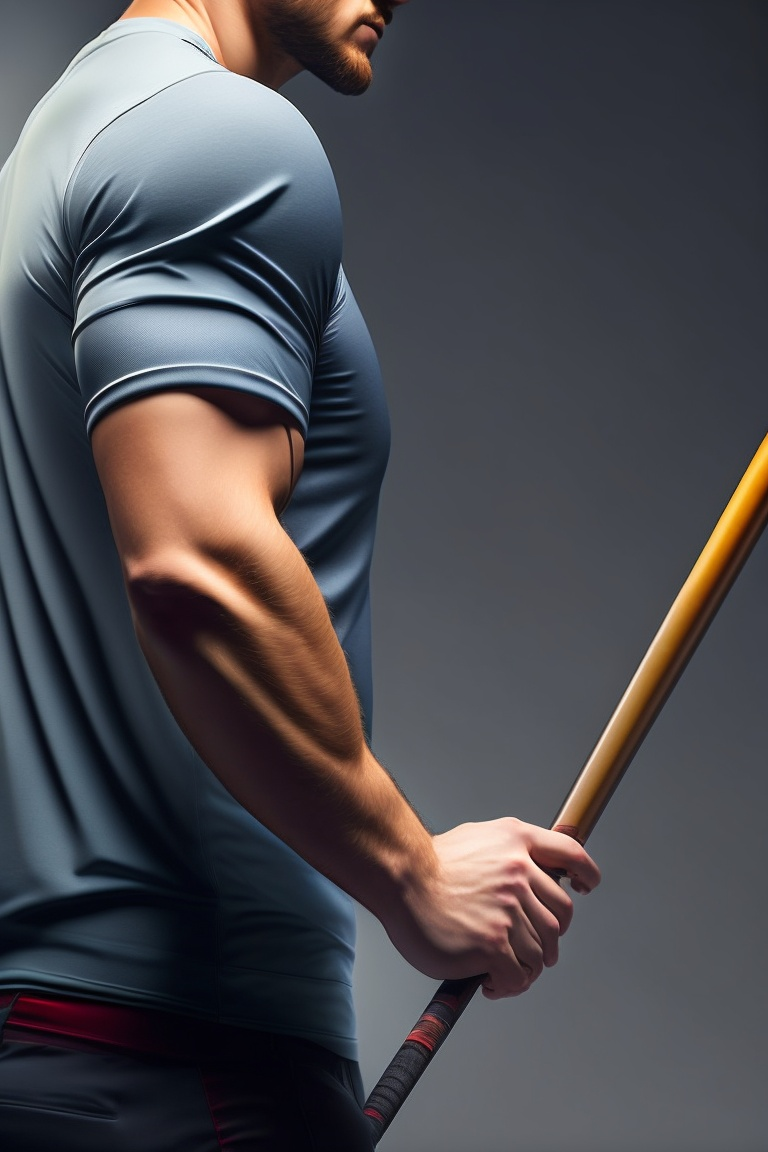
\includegraphics[width=0.4\textwidth]{model/arm.jpeg}
            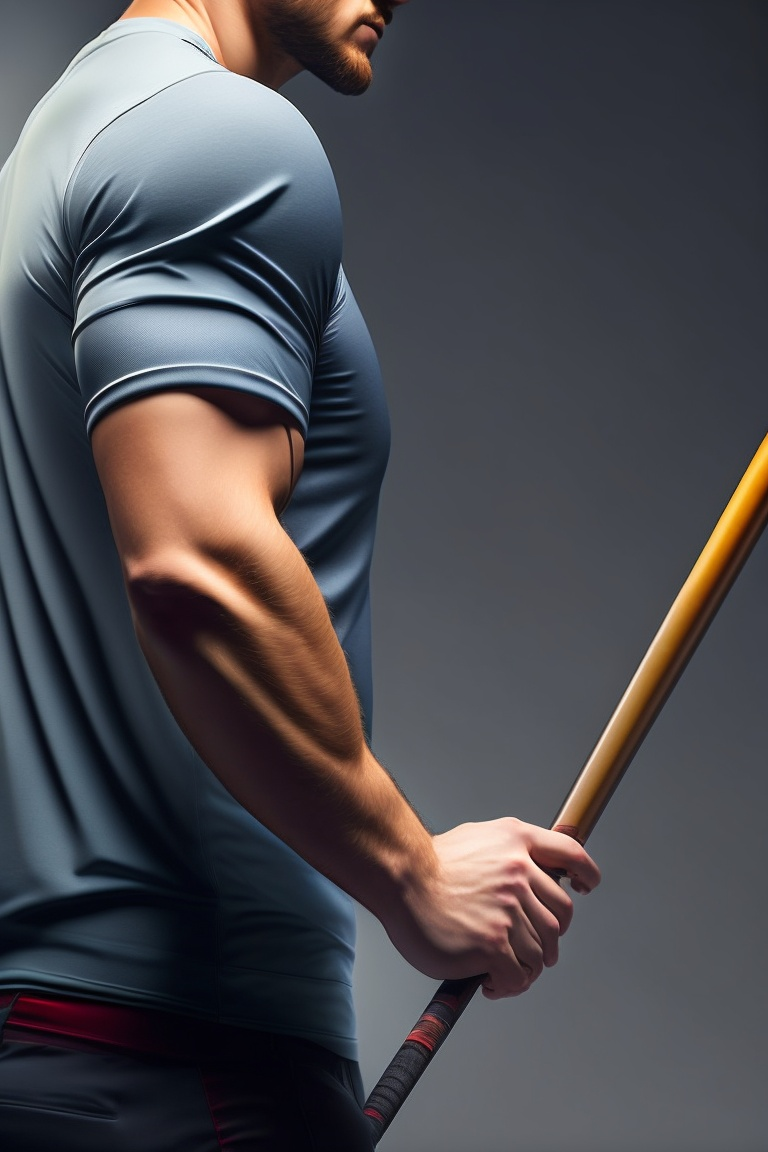
\includegraphics[width=0.4\textwidth]{model/arm.jpeg}
        \end{center}
        \caption{
            Иллюстрация предложенной модели.
            Рисунок слева сгенерирован нейросетью \textit{Lexica Aperture} по текстовому запросу и приведен для визуального соответствия сочленений маятника на схеме с частями тела человека.
        }
        \label{img:arm-model}
    \end{figure}
    


    \ifSubfilesClassLoaded{
        \nocite{*}
        \clearpage
        \bibliographystyle{plain}
        \bibliography{../../refs}
    }{}
\end{document}